\def\VCDate{2015/11/13}\def\VCVersion{(Current)}
\documentclass{article}
\usepackage[screen]{geometry}
\usepackage{ProofPower,graphicx,multicol}
\setlength{\columnsep}{1cm}
\usepackage[metapost,truebbox]{mfpic}
\opengraphsfile{lab4}
\begin{document}
\section{Algorithm}
\begin{multicols}{2}
\begin{mfpic}[72]{-1}{2}{-2}{3}
\tlabeljustify{cc}
\tlpathsep{3pt}
\gfill[yellow]\tlabeloval(0,2.5){decimal-binary conversion}
\tlabelrect(0,2){divide by 2}
\arrow\polyline{(0,1.9), (0,1.1)}
\polygon{(-0.6,0),(0,0.5),(0.6,0),(0,-0.5)}
\tlabelrect(0,1){record quotient and remainder}
\arrow\polyline{(0,0.9), (0,0.5)}
\tlabel(0,0){is quotient zero?}
\tlabel(0.1,-0.6){Yes}
\arrow\polyline{(0.6,0),(1.3,0),(1.3,2),(0.4,2)}
\tlabel(0.7,0.1){No}
\arrow\polyline{(0,-0.5), (0,-0.9)}
\tlabelrect(0,-1){collect remainders right-to-left}
\end{mfpic}
\columnbreak
\\
\textbf{Examples}
\\
\begin{tabular}{ccc}
Division & Quotient & Remainder \\
95/2 & 47 & 1 \\
47/2 & 23 & 1 \\
23/2 & 11 & 1 \\
11/2 & 5 & 1 \\
5/2 & 2 & 1 \\
2/2 & 1 & 0 \\
1/2 & 0 & 1 \\
\end{tabular}
\\ \\ \\Collect remainders from bottom to top
\\$\Rightarrow$ \( 95_{d} = 1011111_{b}\)
\\ \\ \\ \\
\begin{tabular}{ccc}
Division & Quotient & Remainder \\
10/2 & 5 & 0 \\
5/2 & 2 & 1 \\
2/2 & 1 & 0 \\
1/2 & 0 & 1 \\
\end{tabular}
\\ \\ \\Collect remainders from bottom to top
\\$\Rightarrow$ \( 10_{d} = 1010_{b}\)
\end{multicols}
\clearpage
\section{SML}
Implementing this algorithm in SML. If n is zero, return an empty list of digits, otherwise divide by 2 and append the remainder to the list
\begin{GFT}{SML}
\+PolyML.print\_depth 100;\\
\+(* fun dec\_to\_bin 0 = []\\
\+    |dec\_to\_bin n = dec\_to\_bin(n div 2) @ [n mod 2]; *)\\
\+fun cons (x,lst) = (op ::)(x,lst);\\
\+(* fun dec\_to\_bin 0 = []\\
\+   |dec\_to\_bin n = dec\_to\_bin(op div)(n,2) @ cons(op mod)(n,2), []); *)\\
\+fun append (lst1, lst2) = (op @)(lst1, lst2);\\
\+fun dec\_to\_bin 0 = []\\
\+   |dec\_to\_bin n = \\
\+      append(dec\_to\_bin( (op div)(n,2) ), cons((op mod)(n,2), []));\\
\+fun lst\_to\_str (0::xs) = "0" \Circumflex{} lst\_to\_str xs\\
\+   |lst\_to\_str (1::xs) = "1" \Circumflex{} lst\_to\_str xs\\
\+   |lst\_to\_str \_ = "";\\
\+lst\_to\_str(dec\_to\_bin 95); (* expect "1011111" *)\\
\+dec\_to\_bin 10;\\
\+dec\_to\_bin 4096;\\
\+lst\_to\_str(dec\_to\_bin 5000000000); \\
\end{GFT}
\pagebreak
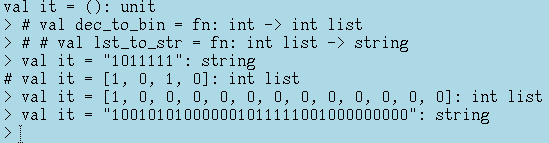
\includegraphics[scale=0.8]{lab4sml.png}
\clearpage\section{C implementation}
To implement this in C, we need to create a structure to represent each digit and a pointer to the next structure node. Every time we need to add another digit, we allocate memory for a new node and fill with the value and set the pointer at end of current list to point to this node.
\begin{GFT}{C source code written to file lab4.c}
\+\#include <stdio.h>\\
\+\#include <stdlib.h>\\
\+typedef struct list\_struct\\
\+\{\\
\+  int list\_head;\\
\+  struct list\_struct * list\_tail;\\
\+\} * int\_list;\\
\+\\
\+int\_list cons(int, int\_list);\\
\+int\_list cons2(int, int\_list);\\
\+void print\_list(int\_list);\\
\+int\_list append(int\_list, int\_list);\\
\+int\_list append2(int\_list, int\_list);\\
\+int\_list dec\_to\_bin(int n);\\
\+int\_list dec\_to\_bin2(int n);\\
\+int\_list EAX;\\
\end{GFT}
\pagebreak
The main function is used to test the algorithm by using a few values such as 95, 10, and 4096.
\begin{GFT}{C source code appended to file lab4.c}
\+int main()\\
\+\{\\
\+ /*\\
\+  int\_list intLst1 = cons(4,cons(3,cons(2,cons(1,NULL))));\\
\+  int\_list intLst2 = cons(8,cons(6,cons(7,cons(5,NULL))));\\
\+  print\_list(append(intLst1,intLst2)); \\
\+\\
\+  append2(intLst1, intLst2);\\
\+  print\_list(EAX);\\
\+  print\_list(dec\_to\_bin(95));\\
\+  */\\
\+  dec\_to\_bin2(95); //assumes EAX global variable has result\\
\+  print\_list(EAX);\\
\+\\
\+  dec\_to\_bin2(10); //assumes EAX global variable has result\\
\+  print\_list(EAX);\\
\+\\
\+  dec\_to\_bin2(4096); //assumes EAX global variable has result\\
\+  print\_list(EAX);\\
\+\}\\
\+\\
\end{GFT}
\pagebreak
Convert decimal to binary using append and cons.
\begin{GFT}{C source code appended to file lab4.c}
\+int\_list dec\_to\_bin(int n)\\
\+\{\\
\+  if(n ==0) return NULL;//empty list\\
\+  else return append(dec\_to\_bin(n/2), cons(n\%2,NULL));\\
\+\}\\
\end{GFT}
This version of dec\_to\_bin does not use function composition so it will be a better model for our conversion to asm code.
\begin{GFT}{C source code appended to file lab4.c}
\+int\_list dec\_to\_bin2(int n)\{\\
\+  int\_list EBX;\\
\+  int quotient, remainder;\\
\+  if(n ==0) EAX = NULL;//empty list\\
\+  else \\
\+  \{ //quotient = n/2; //or shift right one bit\\
\+    quotient = n >> 1;\\
\+    dec\_to\_bin2(quotient);\\
\+    EBX = EAX;\\
\+    remainder = n\%2; // or shift right and check carry flag\\
\+    cons2(remainder, NULL); //returns result in EAX\\
\+    append2(EBX, EAX);     //returns result in EAX\\
\+  \}\\
\+\}\\
\end{GFT}
\pagebreak
Building up a list requires dynamic memory allocation. Let's not worry about freeing that memory (yet). We can create the memory using malloc and put that new element in an existing list.
\begin{GFT}{C source code appended to file lab4.c}
\+int\_list cons(int i, int\_list p)\\
\+\{\\
\+  int\_list lst = malloc( sizeof(struct list\_struct));\\
\+  lst->list\_head = i;\\
\+  lst->list\_tail = p;\\
\+  return lst;\\
\+\}\\
\end{GFT}
Here is a version of cons that does not return a value, but puts result in EAX
\begin{GFT}{C source code appended to file lab4.c}
\+int\_list cons2(int i, int\_list p)\\
\+\{\\
\+  int\_list lst = malloc (sizeof(struct list\_struct));\\
\+  lst->list\_head = i;\\
\+  lst->list\_tail = p;\\
\+  EAX = lst;\\
\+\}\\
\end{GFT}
\pagebreak
To print out a linked list we must loop through all elements until we detect the last one (that is NULL). We can't use a "for" loop since we don't know how many are in the list.
\begin{GFT}{C source code appended to file lab4.c}
\+void print\_list(int\_list lst)\\
\+\{\\
\+  if(lst != NULL)\\
\+  \{\\
\+    printf("\%i",lst->list\_head);\\
\+    print\_list(lst->list\_tail);\\
\+  \}\\
\+  else\\
\+    printf("\Backslash{}n");\\
\+\}\\
\end{GFT}
To append one list to another, use cons and recursively append each element of first list to tail of second list.
\begin{GFT}{C source code appended to file lab4.c}
\+int\_list append(int\_list lst1, int\_list lst2)\\
\+\{\\
\+  if (lst1 != NULL) \\
\+  \{\\
\+     return cons(lst1->list\_head,append(lst1->list\_tail, lst2));\\
\+  \}\\
\+  else\\
\+    return lst2;\\
\+\}\\
\end{GFT}
\pagebreak
Here is a version of append tht is more like asm code. i.e. return is to global (register) variable, and there is no function composition, so we need to call append recursively before calling cons.
\begin{GFT}{C source code appended to file lab4.c}
\+int\_list append2(int\_list lst1, int\_list lst2)\\
\+\{\\
\+  if (lst1 != NULL)\\
\+  \{\\
\+    append2(lst1->list\_tail, lst2);\\
\+    EAX = cons(lst1->list\_head,EAX);\\
\+  \}\\
\+  else \\
\+    EAX = lst2;\\
\+\}\\
\end{GFT}
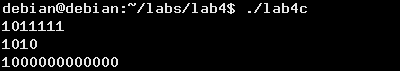
\includegraphics[scale=0.8]{lab4c.png}
\clearpage\section{ASM implementation}
\begin{GFT}{asm source code written to file lab4.s}
\+.data \\
\+  .equ NODESIZE,8\\
\+  .lcomm int\_list,NODESIZE\\
\end{GFT}
\subsection{main function}
This is main function where program start, it will push 2, 95, 10, 4096 to pass parameter to and call function dec\_to\_bin. We also need call printf to print out the results. 
\begin{GFT}{asm source code appended to file lab4.s}
\+.text\\
\+.globl \_start\\
\+\_start:\\
\end{GFT}
\begin{multicols}{2}
Convert 2 decimal to binary
\begin{GFT}{asm source code appended to file lab4.s}
\+  push \$2\\
\+  call dec\_to\_bin		\\
\+\#expect result in EAX\\
\+  add \$4, \%esp\\
\+  push \%eax\\
\+  call print\_list\\
\+  add \$4, \%esp\\
\end{GFT}
\columnbreak
Convert 95 decimal to binary
\begin{GFT}{asm source code appended to file lab4.s}
\+  push \$95\\
\+  call dec\_to\_bin		\\
\+  add \$4, \%esp\\
\+  push \%eax\\
\+  call print\_list\\
\+  add \$4, \%esp\\
\end{GFT}
\end{multicols}
\pagebreak
\begin{multicols}{2}
Convert 10 decimal to binary
\begin{GFT}{asm source code appended to file lab4.s}
\+push \$10\\
\+  call dec\_to\_bin		\\
\+  add \$4, \%esp\\
\+  push \%eax\\
\+  call print\_list\\
\+  add \$4, \%esp\\
\end{GFT}
\columnbreak
Convert 4096 decimal to binary
\begin{GFT}{asm source code appended to file lab4.s}
\+push \$4096\\
\+  call dec\_to\_bin		\\
\+  add \$4, \%esp\\
\+  push \%eax\\
\+  call print\_list\\
\+  add \$4, \%esp\\
\+  mov \$1, \%eax\\
\+  mov \$0, \%ebx\\
\+  int \$0x80\\
\end{GFT}
\end{multicols}
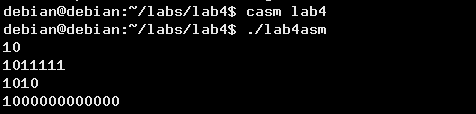
\includegraphics{lab4asm.png} \\
\clearpage\subsection{cons function}
\begin{multicols}{2}
Here is the cons function translated from function con2 of C code. Since we need to use the register EBX for easy copy data, we use push and pop EBX in function to save old value stored in EBX.
\begin{GFT}{asm source code appended to file lab4.s}
\+cons:\\
\+  push \%ebp\\
\+  mov \%esp, \%ebp\\
\+  push \$8		\\
\+  call malloc\\
\+  add \$4, \%esp  	\# expect address in eax\\
\end{GFT}
call malloc function from C library to create 8-bytes size block and return eax point to address of that block. I think we can choose whatever value for size of malloc, as long as eax points to new location generated by malloc function. We choose 8 because it represents that each node have 2 parts: head and tail.
\columnbreak
\begin{GFT}{asm source code appended to file lab4.s}
\+  push \%ebx\\
\+  mov 12(\%ebp), \%ebx 	\#i\\
\+  mov \%ebx, (\%eax) 	\#head\\
\end{GFT}
indirect addressing mode, which means copy the value (i) from EBX to the location in memory where EAX point to
\begin{GFT}{asm source code appended to file lab4.s}
\+  mov 8(\%ebp), \%ebx 	\#p\\
\+  mov \%ebx, 4(\%eax) 	\#tail\\
\+  pop \%ebx\\
\+  mov \%ebp, \%esp\\
\+  pop \%ebp\\
\+  ret\\
\end{GFT}
\end{multicols}
\pagebreak
\subsection{append function}
To append to 2 list together. The first node of new list is the first node of list 1 and end node of new list is the end node of list 2.
\begin{multicols}{2}
\begin{GFT}{asm source code appended to file lab4.s}
\+append:\\
\+ push \%ebp\\
\+ mov \%esp, \%ebp\\
\+ push \%ebx\\
\+ mov 12(\%ebp), \%ebx 	\# ebx = address of lst1\\
\+ cmp \$0, \%ebx	 	\# lst1 == NULL\\
\+ jne if\_append\\
\end{GFT}
If lst1 (first parameter) is equal to NULL, 
\begin{GFT}{asm source code appended to file lab4.s}
\+ mov 8(\%ebp), \%ebx\\
\+ mov \%ebx, \%eax\\
\+ jmp end\_append\\
\end{GFT}
If lst1 (first parameter) is not equal to NULL, call append function again with first parameter is the address that is 4 bytes adding to the address of lst1, and second parameter still the same (lst2).
\columnbreak
\begin{GFT}{asm source code appended to file lab4.s}
\+if\_append:\\
\+ push 4(\%ebx)		\# lst1->tail\\
\+ push 8(\%ebp) 		\# lst2\\
\+ call append\\
\+ add \$8, \%esp\\
\end{GFT}
After call append, call cons to connect new list to where EAX point to, with first parameter is lst1 $\rightarrow$ head and second parameter is EAX, or actually the location where EAX points to.
\begin{GFT}{asm source code appended to file lab4.s}
\+ push (\%ebx)\\
\+ push \%eax\\
\+ call cons	\\
\+ add \$8, \%esp\\
\+end\_append:\\
\+ pop \%ebx\\
\+ mov \%ebp, \%esp\\
\+ pop \%ebp\\
\+ ret\\
\end{GFT}
\end{multicols}
\pagebreak
\subsection{dec\_to\_bin function}
dec\_to\_bin function implementation. Since we need 2 local variable, quotient and remainder, we will sub 8 from ESP to create rooms for them.
\begin{GFT}{asm source code appended to file lab4.s}
\+dec\_to\_bin: \\
\+  push \%ebp\\
\+  mov \%esp, \%ebp\\
\+  sub \$8,\%esp 		\# room for 2 local variables\\
\+  \\
\+  cmp \$0, 8(\%ebp) 	\# n == 0\\
\+  jne else\_part\\
\end{GFT}
If n equals 0, set EAX equal to 0, which mean NULL (or empty list)
\begin{GFT}{asm source code appended to file lab4.s}
\+  mov \$0, \%eax		\# empty list\\
\+  jmp end\_func\\
\end{GFT}
If n is not equal to 0,we copy value n to EAX, then copy value in EAX to first local variable, which is for quotient. The reason we cannot copy value n directly to first local variable is because mov command can't take too many memory references. Then, shift right 1 bit the value stored in first local variable (quotient), which is the same as dividing it by 2. Then push quotient to stack for calling dec\_to\_bin.
\begin{GFT}{asm source code appended to file lab4.s}
\+else\_part:\\
\+  mov 8(\%ebp),\%eax\\
\+  mov \%eax,-4(\%ebp) 	\# copying n to quotient\\
\+  shrl -4(\%ebp) 	\# divide quotient by 2\\
\+  push -4(\%ebp)\\
\+  call dec\_to\_bin\\
\+  add \$4, \%esp\\
\+  push \%ebx\\
\+  mov \%eax, \%ebx	\# EBX = EAX\\
\end{GFT}
Push and pop EBX to save old EBX value after we done calling function.
The second local variable is remainder from dividing n by 2. We can shift right 1 bit and check carry flag (CF). Since we already do shr before, it is not right to do shr again to check CF. Hence, we have to replace local varibale quotient by the number before we did shr, and do shr again to check CF. Use command jnc to check whether CF is 0 or not. If CF = 0, then remainder = n%2 ==0, otherwise, remainder = 1
\begin{GFT}{asm source code appended to file lab4.s}
\+  movl \$0, -8(\%ebp)		\# remainder =0\\
\+  mov 8(\%ebp),\%ecx\\
\+  mov \%ecx,-4(\%ebp) 		\# copying n to quotient\\
\+  shrl -4(\%ebp) 		\# divide quotient by 2\\
\+  jnc call\_cons\\
\+  movl \$1, -8(\%ebp) 		\# remainder = 1\\
\end{GFT}
\pagebreak
Calling cons function with the first parameter is the remainder, second paramter is NULL
\begin{GFT}{asm source code appended to file lab4.s}
\+call\_cons:\\
\+  push -8(\%ebp) 		\# remainder\\
\+  push \$0  			\# NULL\\
\+  call cons			\# expect result in EAX\\
\+  add \$8, \%esp\\
\end{GFT}
call append with 2 parameter EBX and EAX to connect nodes.
\begin{GFT}{asm source code appended to file lab4.s}
\+  push \%ebx\\
\+  push \%eax\\
\+  call append\\
\+  add \$8, \%esp			\# expect result in EAX\\
\+end\_func:\\
\+  pop \%ebx\\
\+  mov \%ebp, \%esp\\
\+  pop \%ebp\\
\+  ret\\
\+\\
\end{GFT}
\pagebreak
\subsection{Print\_list function}
\begin{multicols}{2}
Here is the implementation for print\_list function. fmt string is needed for printing out head value of each node, and fmt2 string for ending print\_list function calling.
\begin{GFT}{asm source code appended to file lab4.s}
\+.data \\
\+  fmt: .string "\%i"\\
\+  fmt2: .string "\Backslash{}n"\\
\+.text\\
\+print\_list:\\
\+  push \%ebp\\
\+  mov \%esp, \%ebp\\
\+  push \%ebx\\
\+  mov 8(\%ebp), \%ebx 		\# parameter\\
\+  cmp \$0, \%ebx\\
\+  je else\_print\\
\end{GFT}
If the list is NULL, print nothing; or else, print out first node's head of the list. 
\\ \textit{push (\%ebx)} means we want to push the value store at location where EBX points to, not the value stored in EBX itself (remember that the value stored in EBX is the address of the first node of the list where EAX points to).
\begin{GFT}{asm source code appended to file lab4.s}
\+  push (\%ebx)\\
\+  push \$fmt\\
\+  call printf\\
\+  add \$8, \%esp\\
\end{GFT}

Then calling function print\_list again with the parameter is the address of the head of second node ( or tail of first node).
\begin{GFT}{asm source code appended to file lab4.s}
\+  push 4(\%ebx)\\
\+  call print\_list\\
\+  add \$4, \%esp\\
\+  jmp end\_print\\
\+\# print out "\Backslash{}n" if reach the end of the list\\
\+else\_print:\\
\+  push \$fmt2\\
\+  call printf\\
\+  add \$4, \%esp\\
\+end\_print:\\
\+  pop \%ebx\\
\+  mov \%ebp, \%esp\\
\+  pop \%ebp\\
\+  ret\\
\end{GFT}
\end{multicols}
\clearpage\section{Stack Frame}
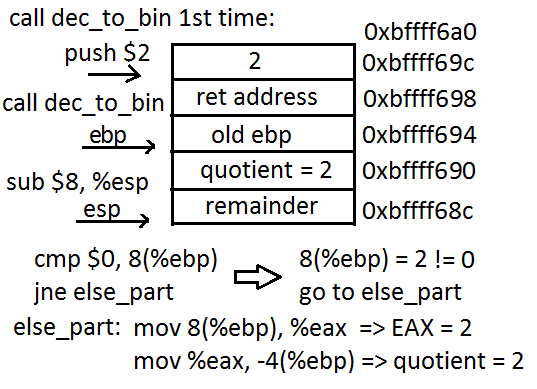
\includegraphics[scale=0.5]{stack1.png}
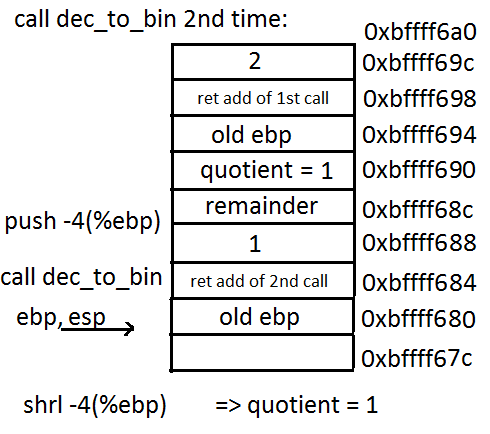
\includegraphics[scale=0.5]{stack2.png}\\ \\ 
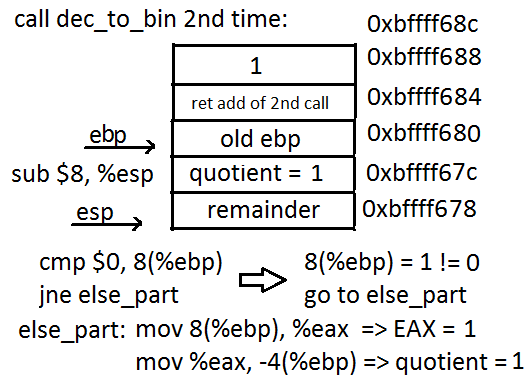
\includegraphics[scale=0.5]{stack3.png}
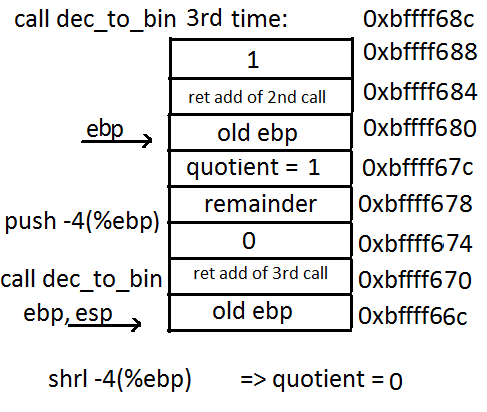
\includegraphics[scale=0.5]{stack4.png}\\
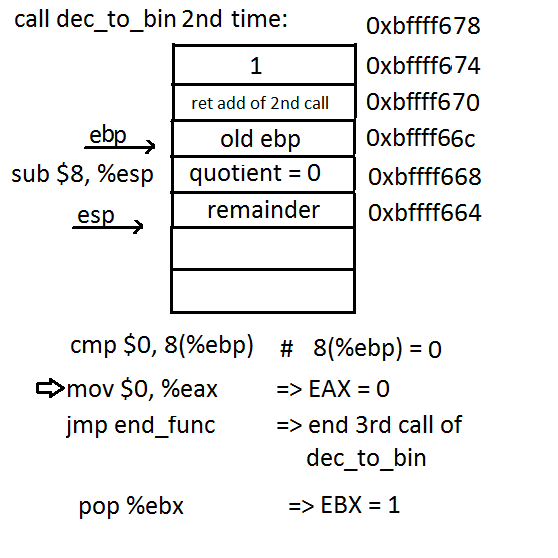
\includegraphics[scale=0.5]{stack5.png}
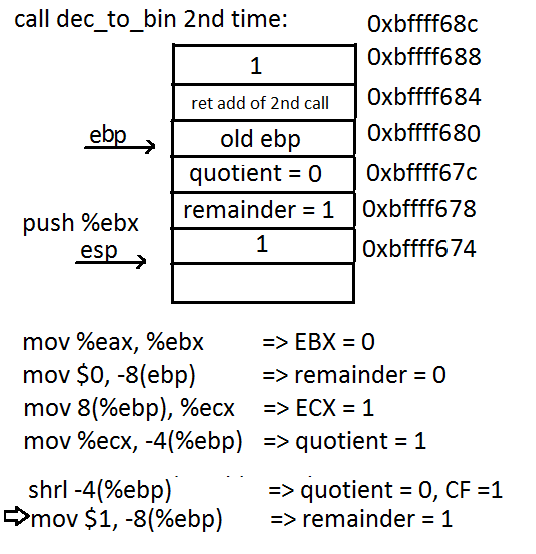
\includegraphics[scale=0.5]{stack6.png}\\ \\ 
\begin{center}
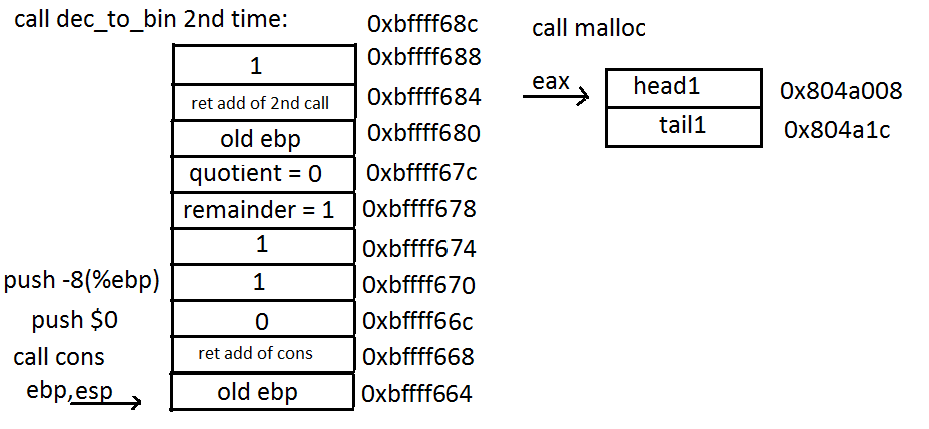
\includegraphics[scale=0.5]{stack7.png} \\
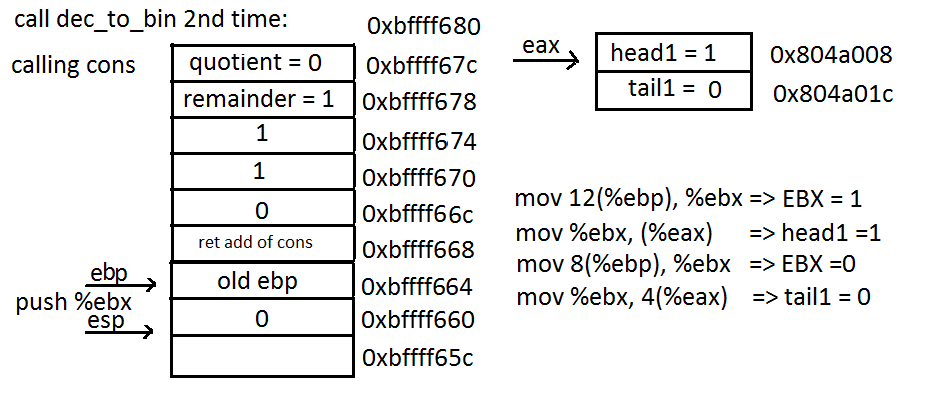
\includegraphics[scale=0.5]{stack8.png} \\
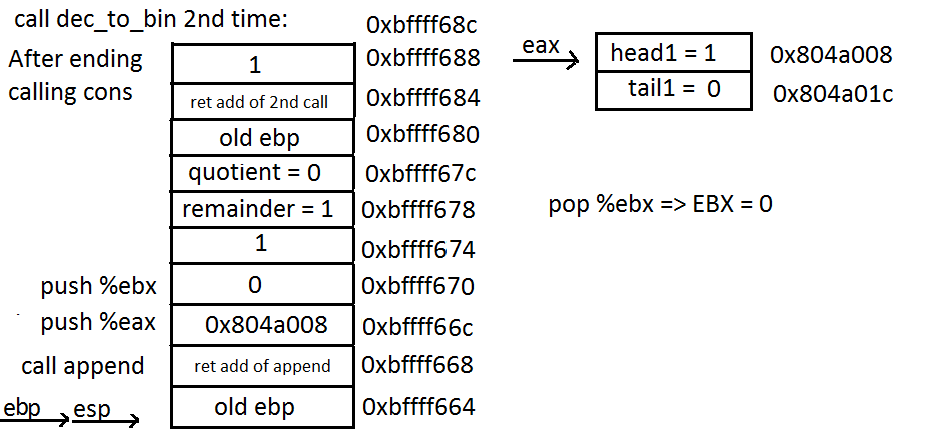
\includegraphics[scale=0.5]{stack9.png} \\
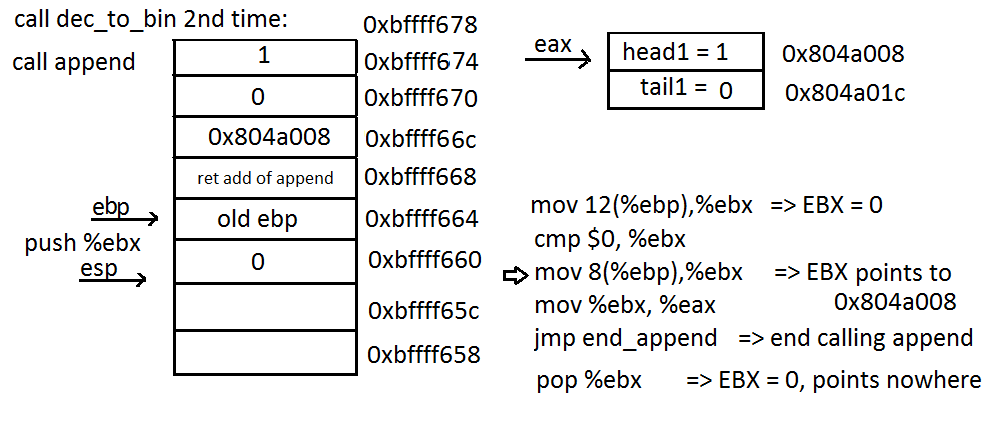
\includegraphics[scale=0.5]{stack10.png}\\
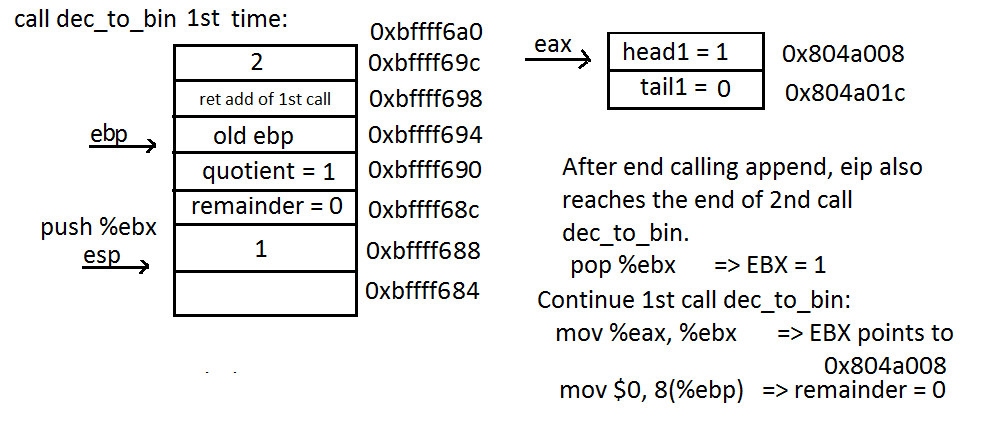
\includegraphics[scale=0.5]{stack11.png} \\
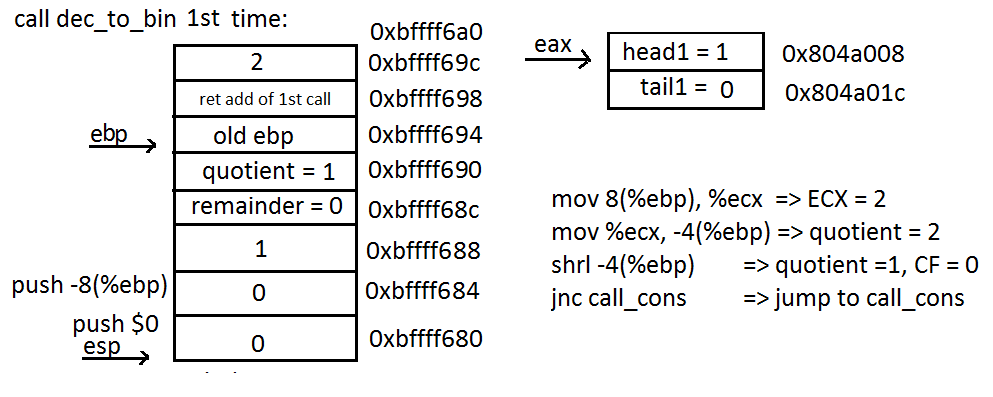
\includegraphics[scale=0.5]{stack12.png}\\
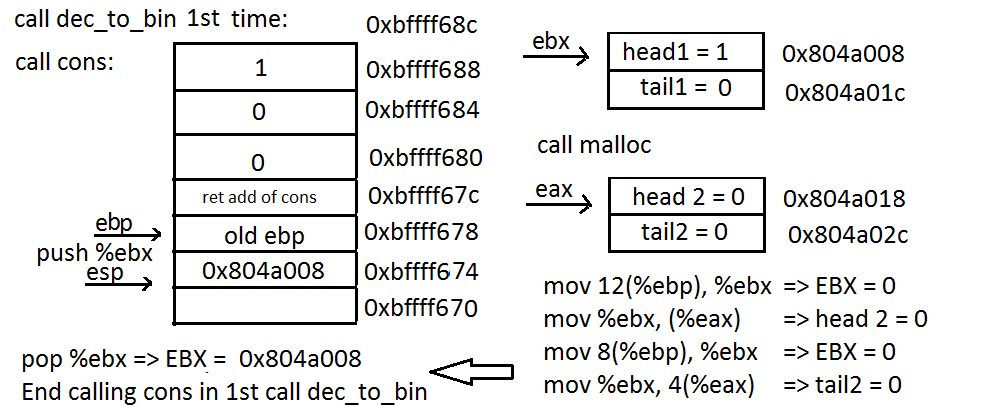
\includegraphics[scale=0.5]{stack13.png} \\
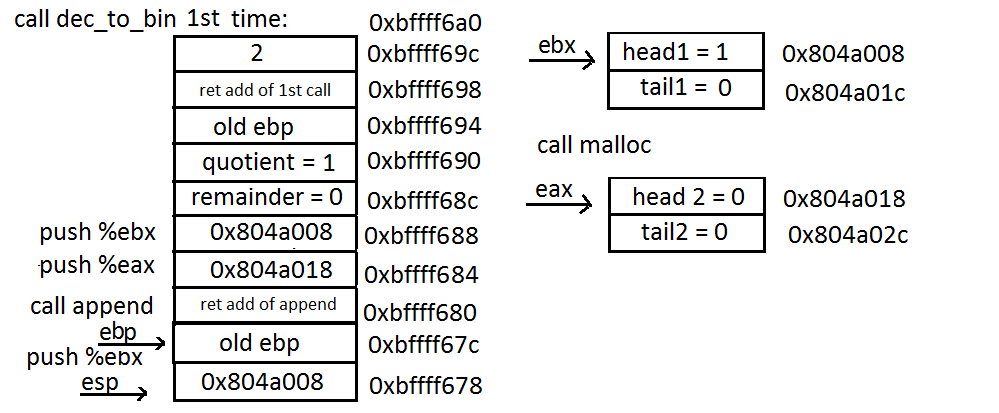
\includegraphics[scale=0.5]{stack14.png}\\
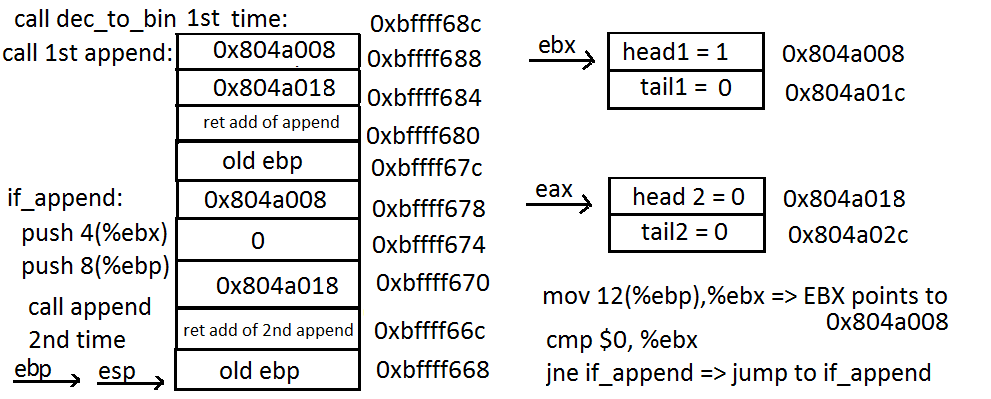
\includegraphics[scale=0.5]{stack15.png} \\
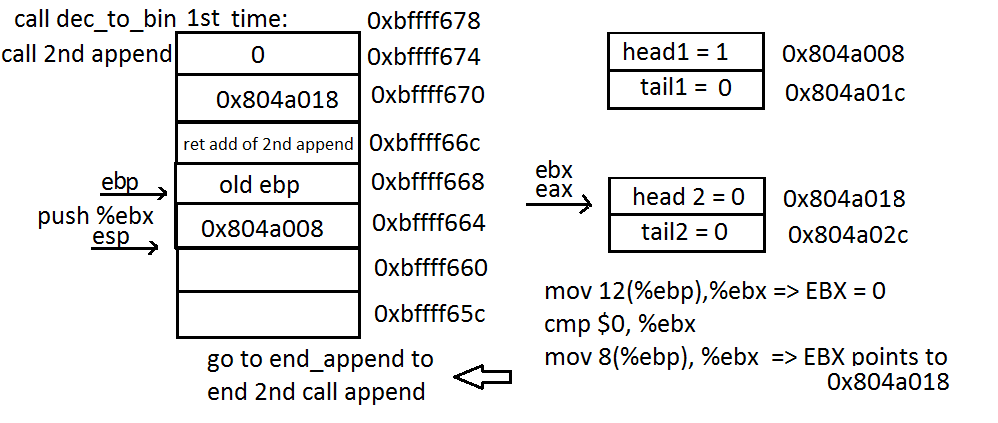
\includegraphics[scale=0.5]{stack16.png}\\
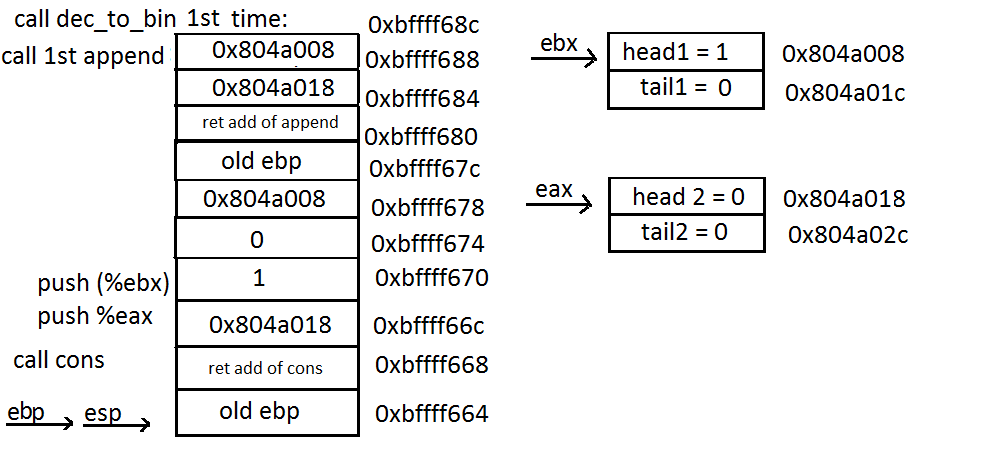
\includegraphics[scale=0.5]{stack17.png} \\
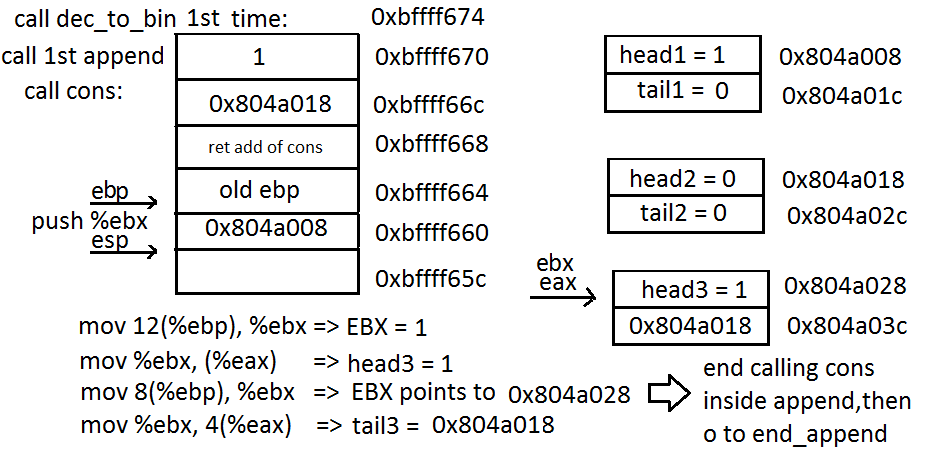
\includegraphics[scale=0.5]{stack18.png} \\
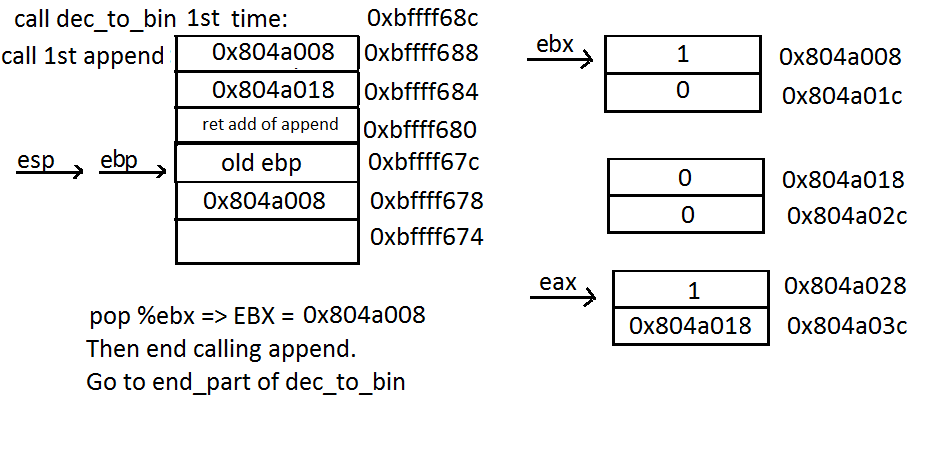
\includegraphics[scale=0.5]{stack19.png} \\
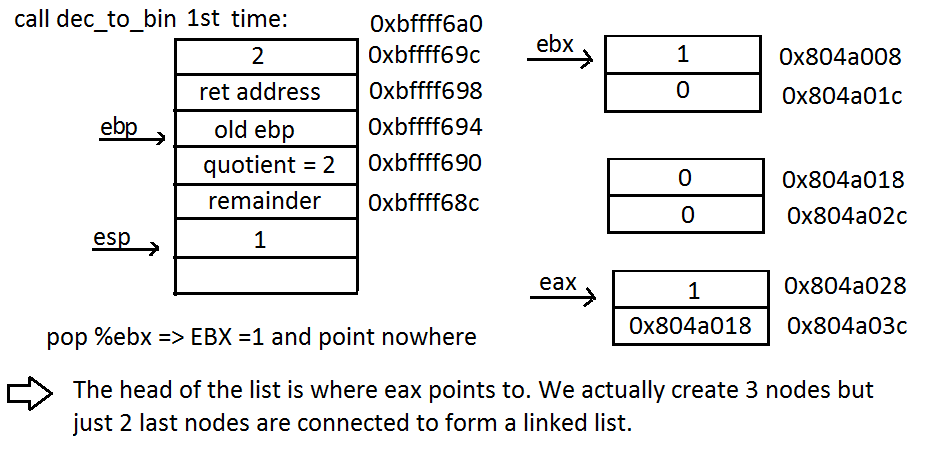
\includegraphics[scale=0.5]{stack20.png}
\end{center}
\end{document}
